\documentclass[fontset=windows]{article}
\usepackage{My}

\begin{document}

\section{从数据文件读取数据绘图}
%% 从数据文件读取数据绘图
\begin{tikzpicture}
	\begin{axis}
	\addplot3[surf,mesh/ordering=y varies]
	table {concat_VV_together.dat};
	\end{axis}
	\end{tikzpicture}


\section{普通二位函数绘制}
\begin{Plot}{scale=0.8}{>=stealth}
	\plot{blue!40, thick}{-1:4}{\x*\x-2*\x-1}
	\plot{red, thick}{0:pi}{3*sin(\x r)}
\end{Plot}


\section{极坐标图形绘制}
\polarplot{scale=0.2}{cyan, domain=0:1440}{0.01/pi*\t}
\polarplot{scale=2}{red, domain=0:720}{sin(2*\t)}

\section{参数方程的绘制}
\subsection{三维参数方程}
\paraplotz{scale=0.5} {{sin(deg(t))},{cos(deg(t))},{t}} {}{view = {60}{90}, hide axis}
\paraplotz{scale=0.5}{{sin(deg(t))},{cos(deg(t))},{t}}{}{view = {90}{30}}
\paraplotz{scale=0.5}{{sin(deg(t))},{cos(deg(t))},{t}}{thick, red}{view = {60}{30}, axis lines = center, }

\subsection{二维参数方程}
\paraplot{scale=1}{{10*cos(t)}, {sin(t)}}{thick, color=blue}{hide axis}

\section{三维曲面绘制}
\subsection{mesh方法}
%% mesh
\begin{tikzpicture}
    \begin{axis}[
    	title = 我是title,
    	hide axis,		%% 隐藏坐标轴
    	colormap/cool	%% 指定色系
    ]
        \addplot3[mesh, samples=50, domain=-8:8]{x*y/(x^2+y^2)};
        \addlegendentry{$\frac{\sin(r)}{r}$}	%% 添加图例
    \end{axis}
\end{tikzpicture}

\subsection{默认方法}
\begin{tikzpicture}
    \begin{axis}[
    	title = 我是title,
    	hide axis,		%% 隐藏坐标轴
    	colormap/cool	%% 指定色系
    ]
        \addplot3[samples=50, domain=-8:8]{sin(deg(sqrt(x^2+y^2)))/sqrt(x^2+y^2)};
        \addlegendentry{$\frac{\sin(r)}{r}$}	%% 添加图例
    \end{axis}
\end{tikzpicture}

\subsection{surf方法}
\plotz{}{sin(deg(sqrt(x^2+y^2)))/sqrt(x^2+y^2)}{surf}{}{图例}

\subsection{TikZ中的旋转命令}
\begin{center}
	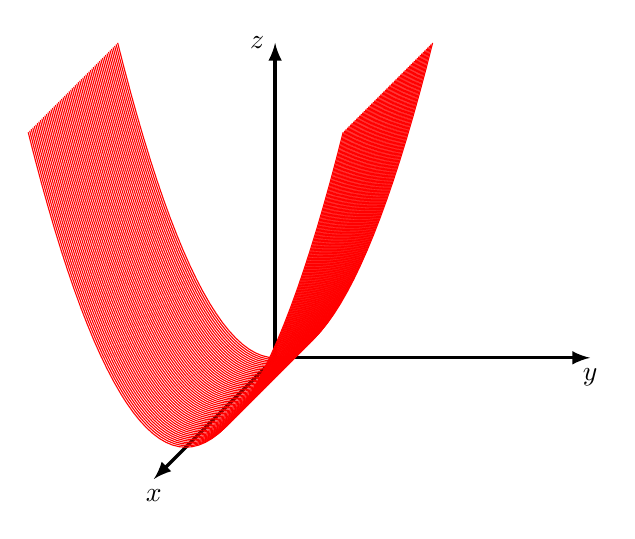
\begin{tikzpicture}
		\coordinate (O) at (0,0,0);
		\draw[very thick, ->, >=latex] (O) -- (4,0,0) node[below]{\(y\)};
		\draw[very thick, ->, >=latex] (O) -- (0,4,0) node[left]{\(z\)};
		\draw[very thick, ->, >=latex] (O) -- (0,0,4) node[below]{\(x\)};
		
		\foreach \z in {0,0.05, ..., 3}{
			\draw[red, domain=0:2] plot (\x,\x*\x,\z);
			\draw[red, domain=0:2] plot (-\x,\x*\x,\z);
		}
	\end{tikzpicture}

	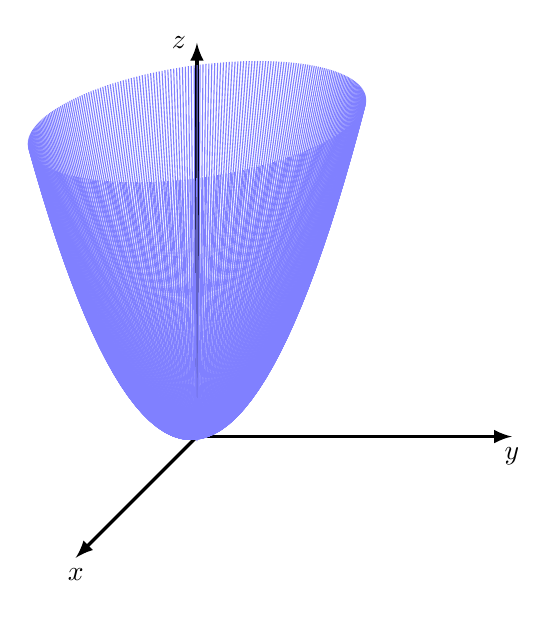
\begin{tikzpicture}
		\coordinate (O) at (0,0,0);
		\draw[very thick, ->, >=latex] (O) -- (4,0,0) node[below]{\(y\)};
		\draw[very thick, ->, >=latex] (O) -- (0,5,0) node[left]{\(z\)};
		\draw[very thick, ->, >=latex] (O) -- (0,0,4) node[below]{\(x\)};
		
		\foreach \angle in {0, ..., 360}{
			\draw[blue!50, rotate around y=\angle, domain=0:2] plot (\x,\x*\x, 0);
		}
	\end{tikzpicture}
\end{center}
\end{document}






